\lecture

\begin{guiding}
The Thom class lives on the total space of a bundle. Geometry enters through one
observation: a submanifold has a neighbourhood that looks exactly like its
normal bundle. This transports the Thom class into the cohomology of the
ambient manifold, where it becomes the \emph{dual class} of the submanifold.
Applied to the diagonal in $M\times M$ it will compute the Euler class of $TM$.
\end{guiding}

Throughout, $M^n\subset A^{n+k}$ is a closed smooth $n$-manifold embedded in a
smooth Riemannian $(n+k)$-manifold, and
\[
\nu=\big\{v\in T_xA\ \big|\ x\in M,\ v\perp T_xM\big\}
\]
is its normal bundle, so that $TA|_M\iso TM\oplus\nu$.

\section{The tubular neighbourhood theorem}

\begin{theorem}\label{thm:tnt}
There is an open neighbourhood of $M$ in $A$ diffeomorphic to the total space
$E(\nu)$, by a diffeomorphism restricting to the identity on the zero section.
\end{theorem}

\begin{proof}
\begin{strategy}
Write down a map from the normal bundle to $A$ which is the identity on $M$ and
whose differential along $M$ is invertible, then quote the global inverse
function theorem. The map is the exponential map of the Riemannian metric.
\end{strategy}

\step{1} \emph{The inverse function theorem, global form (quoted).} If
$f\colon N\to A$ is smooth, injective on a compact submanifold $M\subset N$, and
$df_x$ is an isomorphism for every $x\in M$, then $f$ maps some neighbourhood of
$M$ in $N$ diffeomorphically onto a neighbourhood of $f(M)$ in $A$.

\step{2} \emph{The exponential map.} For $\eps>0$ let
$E(\eps)=\{v\in E(\nu)\mid |v|<\eps\}$, an open neighbourhood of the zero
section, and define
\[
\mathrm{Exp}\colon E(\eps)\longrightarrow A,
\qquad
(x,v)\longmapsto\gamma_v(1),
\]
where $\gamma_v$ is the unique geodesic with $\gamma_v(0)=x$ and
$\dot\gamma_v(0)=v$. For $\eps$ small this is defined and smooth, by the theory
of ordinary differential equations.

\step{3} \emph{Behaviour along $M$.} On the zero section $\mathrm{Exp}$ is the
identity. Its differential at a point of the zero section, under the canonical
splitting $T\big(E(\nu)\big)\big|_M\iso TM\oplus\nu\iso TA|_M$, is the identity:
the $TM$ directions are unmoved and the $\nu$ directions differentiate the
geodesics, giving back $v$.

\step{4} \emph{Conclusion.} Step 1 applies with $N=E(\eps)$ and $f=\mathrm{Exp}$,
so a neighbourhood of the zero section in $E(\eps)$ maps diffeomorphically onto
a neighbourhood $U$ of $M$ in $A$. Finally $E(\nu)\iso E(\eps)$ by the fibrewise
rescaling $v\mapsto \eps v/\sqrt{1+|v|^2}$.
\end{proof}

\begin{center}
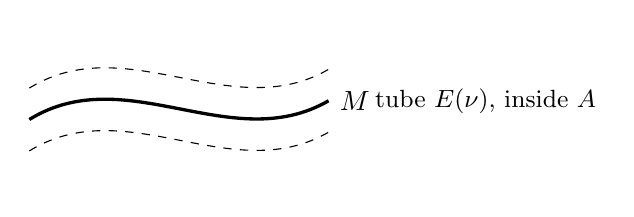
\begin{tikzpicture}[scale=0.95]
\draw[very thick] (0,0) .. controls (1.3,0.8) and (2.7,-0.5) .. (4,0.25);
\node at (4.35,0.25) {$M$};
\draw[dashed] (0,0.42) .. controls (1.3,1.22) and (2.7,-0.08) .. (4,0.67);
\draw[dashed] (0,-0.42) .. controls (1.3,0.38) and (2.7,-0.92) .. (4,-0.17);
\node at (6.1,0.25) {\small tube $\iso E(\nu)$, inside $A$};
\end{tikzpicture}
\end{center}

\begin{corollary}\label{cor:excision-tube}
If $M$ is closed in $A$ then, for any coefficient ring,
\[
H^*\big(E,E_0\big)\ \iso\ H^*\big(A,\,A\smallsetminus M\big),
\qquad E=E(\nu).
\]
\end{corollary}

\begin{proof}
Let $U\subset A$ be a tubular neighbourhood, so $(U,U\smallsetminus M)\iso
(E,E_0)$ by Theorem~\ref{thm:tnt}. Excising the closed set
$A\smallsetminus U$ from the pair $(A,A\smallsetminus M)$ gives
$H^*(A,A\smallsetminus M)\iso H^*(U,U\smallsetminus M)$.
\end{proof}

\section{The dual class of a submanifold}

Assume from now on either $\Z_2$ coefficients, or that $TA$ and $TM$ are
oriented and coefficients are $\Z$; in the latter case $\nu$ inherits an
orientation from $TA|_M\iso TM\oplus\nu$. By Theorem~\ref{thm:thom} there is a
unique Thom class $u\in H^k(E,E_0)$, and Corollary~\ref{cor:excision-tube}
carries it to a class
\[
u'\in H^k\big(A,\,A\smallsetminus M\big),
\]
whose image in $H^k(A)$ we denote $u''$. Both are called the \emph{dual class}
of $M$ in $A$.

\begin{remark}
The class $u'$ does not depend on the Riemannian metric: two metrics $g_1,g_2$
are joined by the path $tg_1+(1-t)g_2$ of metrics, and the corresponding
exponential identifications are homotopic.
\end{remark}

\begin{theorem}\label{thm:dual-restricts-euler}
The inclusions $M\hookrightarrow A\hookrightarrow(A,A\smallsetminus M)$ induce
\[
H^k\big(A,A\smallsetminus M\big)\longrightarrow H^k(A)\longrightarrow H^k(M),
\]
under which $u'\mapsto u''$ and $u''$ restricts to
\[
\begin{cases}
e(\nu)&\text{in the oriented case},\\[2pt]
w_k(\nu)&\text{over }\Z_2 .
\end{cases}
\]
\end{theorem}

\begin{proof}
Restrict the whole picture to the tube. The composite
$H^k(E,E_0)\to H^k(E)\iso H^k(M)$ sends $u$ to $e(\nu)$, by the very definition
of the Euler class; over $\Z_2$ it sends $u$ to $w_k(\nu)$ by
Theorem~\ref{thm:euler-properties}(4). The square
\[
\begin{tikzcd}[row sep=large, column sep=large]
H^k(A,A{\smallsetminus}M)\arrow[r]\arrow[d,"\iso"'] & H^k(A)\arrow[r]\arrow[d]
& H^k(M)\arrow[d,equal]\\
H^k(E,E_0)\arrow[r] & H^k(E)\arrow[r,"\iso"] & H^k(M)
\end{tikzcd}
\]
commutes, since all maps are induced by inclusions and the tubular
identification.
\end{proof}

\begin{corollary}\label{cor:embedding-obstruction}
If $M^n$ is closed and smoothly embedded in $\R^{n+k}$, then $w_k(\nu)=0$, and
in the oriented case $e(\nu)=0$.
\end{corollary}

\begin{proof}
Here $u''$ lies in $H^k(\R^{n+k})=0$ for $k>0$, so its restriction to $M$
vanishes; apply Theorem~\ref{thm:dual-restricts-euler}.
\end{proof}

\begin{example}
Combined with Whitney duality this refines the immersion obstructions of
Lecture 2 into \emph{embedding} obstructions. Since
$\bar w(T\RP^{2^r})=1+a+\dots+a^{2^r-1}$ has non-zero term in degree $2^r-1$,
an embedding $\RP^{2^r}\subset\R^{2^r+k}$ would give
$w_j(\nu)=\bar w_j(T\RP^{2^r})=0$ for $j>k$ and, by
Corollary~\ref{cor:embedding-obstruction}, also $w_k(\nu)=0$; hence
$k\ge 2^r$. So $\RP^{2^r}$ does not embed in $\R^{2\cdot2^r-1}$, which is sharp
against Whitney's embedding theorem $M^n\hookrightarrow\R^{2n}$.
\end{example}

\section{The diagonal}

Apply the machine to the diagonal embedding
$\Delta\colon M\to M\times M$, $x\mapsto(x,x)$, of a closed Riemannian manifold;
the product carries the product metric.

\begin{lemma}\label{lem:normal-diagonal}
The normal bundle $N(\Delta)$ of $\Delta(M)\subset M\times M$ is canonically
isomorphic to $TM$.
\end{lemma}

\begin{proof}
At $(x,x)$ the tangent space of the diagonal is
$T\Delta=\{(v,v)\}\subset T_xM\times T_xM$, whose orthogonal complement is
$N(\Delta)=\{(-v,v)\}$. The map
\[
TM\longrightarrow N(\Delta),
\qquad
(x,v)\longmapsto\big((x,x),\,(-v,v)\big),
\]
is continuous, fibrewise a linear isomorphism, hence an isomorphism of bundles
by Lemma~\ref{lem:fibrewise-iso}.
\end{proof}

\begin{corollary}\label{cor:diagonal-euler}
Let $u''\in H^n(M\times M)$ be the dual class of the diagonal. Then
\[
\Delta^*u''=e(TM)
\qquad\big(\text{resp. } w_n(TM)\ \text{over }\Z_2\big).
\]
\end{corollary}

\begin{proof}
Theorem~\ref{thm:dual-restricts-euler} identifies the restriction of $u''$ to
$\Delta(M)$ with $e(N(\Delta))$, and
Lemma~\ref{lem:normal-diagonal} identifies $N(\Delta)$ with $TM$. Restricting
to $\Delta(M)$ is the same as applying $\Delta^*$.
\end{proof}

The dual class of the diagonal interacts with the product structure very
rigidly.

\begin{lemma}\label{lem:ax1}
For every $a\in H^*(M)$,
\[
(a\times1)\smile u''=(1\times a)\smile u''\ \in H^*(M\times M).
\]
\end{lemma}

\begin{proof}
\begin{strategy}
Both products are computed from classes supported near the diagonal, and near
the diagonal the two projections $M\times M\to M$ agree. Make this precise by
factoring the cup product through the relative group and restricting to a
tubular neighbourhood, which retracts onto the diagonal.
\end{strategy}

\step{1} \emph{Where the product is computed.} Let $U$ be a tubular
neighbourhood of $\Delta(M)$ in $M\times M$. Cup product with the relative class
$u'$ gives a commutative square
\[
\begin{tikzcd}[row sep=large, column sep=large]
H^i(M\times M)\arrow[r]\arrow[d,"\smile u'"'] & H^i(U)\arrow[d,"\smile u'|_U"]\\
H^{i+n}\big(M\times M,\ M\times M\smallsetminus\Delta\big)
\arrow[r,"\iso"',"\text{excision}"] & H^{i+n}(U,\,U\smallsetminus\Delta)
\end{tikzcd}
\]
so $x\smile u'$ depends only on the restriction $x|_U$.

\step{2} \emph{The two restrictions agree.} The diagonal is a deformation
retract of $U$, and $p_1\circ\Delta=p_2\circ\Delta=\mathrm{id}$; hence the two
maps $p_1,p_2\colon U\to M$ are homotopic, and for $a\in H^*(M)$,
\[
(a\times1)\big|_U=p_1^*a\big|_U=p_2^*a\big|_U=(1\times a)\big|_U .
\]

\step{3} \emph{Conclusion.} By Steps 1 and 2,
$(a\times1)\smile u'=(1\times a)\smile u'$ in
$H^*(M\times M,\,M\times M\smallsetminus\Delta)$. Mapping to the absolute group
$H^*(M\times M)$ turns $u'$ into $u''$ and preserves the identity.
\end{proof}

\section{The slant product}

We work with field coefficients, so that $H^*(X\times Y)=H^*(X)\otimes H^*(Y)$.

\begin{definition}
The \emph{slant product}
\[
/\ \colon\ H^{p+q}(X\times Y)\otimes H_q(Y)\longrightarrow H^p(X)
\]
is defined on decomposable classes by
$(\alpha\times\beta)/\mu=\langle\beta,\mu\rangle\,\alpha$ and extended linearly.
\end{definition}

\begin{lemma}\label{lem:slant-identity}
For $a\in H^*(X)$, $P\in H^*(X\times Y)$ and $\mu\in H_*(Y)$,
\[
\big((a\times1)\smile P\big)\big/\mu\ =\ a\smile\big(P/\mu\big).
\]
\end{lemma}

\begin{proof}
Write $P=\sum_{i,j}a_{ij}\,p_i\times q_j$ with $p_i\in H^*(X)$,
$q_j\in H^*(Y)$. Then
\[
(a\times1)\smile P=\sum_{i,j}a_{ij}\,(a\smile p_i)\times q_j ,
\]
so slanting with $\mu$ gives
$\sum_{i,j}a_{ij}\langle q_j,\mu\rangle\,(a\smile p_i)
=a\smile\big(\sum_{i,j}a_{ij}\langle q_j,\mu\rangle\,p_i\big)=a\smile(P/\mu)$.
\end{proof}

\begin{lemma}\label{lem:u-over-mu}
Let $\mu\in H_n(M)$ be the fundamental class. Then
\[
u''/\mu=1\ \in H^0(M).
\]
\end{lemma}

The proof is a local computation which opens the next lecture. Together with
Lemma~\ref{lem:ax1} and Corollary~\ref{cor:diagonal-euler} it will determine
$u''$ completely and produce the identity
$\langle e(TM),\mu\rangle=\chi(M)$.
